\documentclass{../../oss-handout}
\usepackage{newtxmath,newtxtext}
%\usepackage{amsmath}
\usepackage{enumitem}
\usepackage{tikz}
\usepackage{siunitx}
\usepackage{titlesec}

\titleformat{\section}{\fontsize{13}{15}\bfseries}{\thesection}{1em}{}
\titlespacing{\section}{0pt}{14pt}{2pt}

\titleformat{\subsection}{\bfseries}{\thesubsection}{1em}{}
\titlespacing{\subsection}{0pt}{6pt}{-3pt}

\newcommand{\iii}{\hat\imath}
\newcommand{\jjj}{\hat\jmath}

\tikzset{
  >=latex
}

\setlength{\parindent}{0pt}
\setlength{\parskip}{6pt}
\setlength{\headheight}{26pt}


% Set the page style for the document
\pagestyle{plain}

% Course & handout information
\renewcommand{\institution}{Olympiads School}%, Toronto, ON, Canada}
\renewcommand{\coursetitle}{Advanced Placement Physics 1 \& C}
\renewcommand{\term}{Fall 2022}

\title{Projectile Motion}
\author{Dr.\ Timothy Leung}
\date{\today}

\begin{document}
\thispagestyle{title}
\gentitle

\section{General Projectile Motion}
A \textbf{projectile} is an object that is launched with an initial velocity
of $\vec V_0$ at an angle $\theta$ with the horizontal. It travels along a
parabolic trajectory and accelerates only due to gravity, as shown in
Figure~\ref{fig:projectile}. 
\begin{figure}[ht]
  \centering
  \begin{tikzpicture}[scale=1.3]
    \draw[thick,->](0,0)--(2,0) node[right]{$x$};
    \draw[thick,->](0,0)--(0,2) node[above]{$y$};
    \draw[dotted,domain=0:5,thick] plot (\x, {1.2*\x-.2*\x*\x});
    \begin{scope}[ultra thick,->]
      \draw[rotate=atan(1.2)](0,0)--(2,0)node[above]{$\vec V_0$};
      \draw[red] (0,0)--(0,2*sin{atan{1.2}}) node[left]{$\vec v_0$};
      \draw[blue](0,0)--(2*cos{atan{1.2}},0)node[below]{$\vec u_0$};
    \end{scope}
    \draw[thick,->](.8,0)arc(0:atan{1.2}:.8) node[pos=.65,right]{$\theta$};
  \end{tikzpicture}
  \caption{The parameters defining the motion of a projectile.}
  \label{fig:projectile}
\end{figure}

In general, when solving a projectile motion project:
\begin{itemize}[nosep]
\item the $x$-axis ($\iii$ direction) is defined as the \emph{horizontal}
  direction, with the ($+$) direction pointing forward
\item the $y$-axis ($\jjj$ direction) is the \emph{vertical} direction, with
  the ($+$) direction pointing upwards
\item the origin of the coordinate system is where the projectile is launched
\item the launch angle is ($+$) if it is above the horizontal, and ($-$) if it
  is below
\end{itemize}
This set up is consistent with the standard right-handed Cartesian coordinate
system. The initial velocity $\vec V_0$ can be resolved into its $\iii$ and
$\jjj$ components, $\vec u_0$ and $\vec v_0$:
\begin{equation}
  \vec V_0 =\vec u_0+\vec v_0
  =\left[V_0\cos\theta\right]\iii + \left[V_0\sin\theta\right]\jjj
\end{equation}
where $V_0=|\vec V_0|$.

\subsection{Motion in the Horizontal Direction}
There is no acceleration (i.e.\ $a_x=0$) along the $\iii$ direction, therefore
horizontal velocity is a constant $u=u_0$. The kinematic equations are reduce
to a single equation that relates the horizontal position (displacement) $x$ as
a function of time:
\begin{equation}
  x(t)=u_0t=\left[V_0\cos\theta\right] t
  \label{eq:x}
\end{equation}

\subsection{Motion in the Vertical Direction}
There is a constant acceleration due to gravity alone along the $\jjj$
direction, i.e.\ $a_y=-g$. (Acceleration is \emph{negative} due to the fact that
the positive $y$-axis points upwards.) The kinematic equations along the
vertical direction are therefore:
\begin{align}
  y(t) &= \left[V_0\sin\theta\right]t-\frac12gt^2\label{eq:y}\\
  v(t) &= \left[V_0\sin\theta\right] -gt\\
  \left[v(y)\right]^2&=V_0^2\sin^2\theta-2gy
  \label{eq:maxh}
\end{align}

\subsection{Solving Projectile Motion Problem}
For most projectile motion problems, Eqs.~\ref{eq:x} and \ref{eq:y} are the
most often used. Because $\iii$ and $\jjj$ directions are
orthogonal\footnote{In proper language of mathematics, they are therefore
  \emph{linearly independent}.}, horizontal and vertical displacements $x(t)$
and $y(t)$ are independent of each other. However, there are variables that are
shared in both directions, namely:
\begin{itemize}[nosep]
\item Time $t$
\item Launch angle $\theta$
\item Initial speed $V_0$
\end{itemize}
When solving for most projectile motion problems, there likely will be two
unknowns that need to be solved (although you may not be explicitly told what
one of them is), requiring two equations (the $x$ and $y$ kinematic equations).
In some rare cases, if an object lands on an incline, there will be a third
equation describing the relationship between $x$ and $y$ of the incline.

\section{Parabolic Path}
We can easily see that the path of a projectile is entirely parabolic. When
solving for the flight time in the $x$ direction (Eq.~\ref{eq:x}), we get:
\begin{equation}
  t=\frac x{V_0\cos\theta}
  \label{eq:t1}
\end{equation}
Substituting Eq.~\ref{eq:t1} into Eq.~\ref{eq:y}, we have
\begin{align}
  y &=\left(V_0\sin\theta\right) t-\frac12gt^2\nonumber\\
  &= \left(V_0\sin\theta\right)\left(\frac x{V_0\cos\theta}\right)-\frac12g
  \left(\frac x{V_0\cos\theta}\right)^2\nonumber\\
  y&=\left(\tan\theta\right) x-\left(\frac g{2V_0^2\cos^2\theta}\right)x^2
\end{align}
It is clear that the $y$ is quadratic in $x$, and therefore the path is a
parabola.

\section{Projectiles with Symmetric Trajectories}
A \textbf{symmetric trajectory} is a special case of projectile motion where an
object is launched at an angle of $\theta$ (between \ang{0} and \ang{90}) above
the horizontal\footnote{This may be obvious, but angles \emph{below} the 
  horizontal will never have a symmetric trajectory.} and then lands at the
same height. Examples may include hitting a golf ball toward the hole, or
shooting a bullet toward a horizontal target\footnote{Shooting a bullet toward
  a horizontal target always require an upward angle because of gravity.}
\footnote{Note that the equations for symmetric trajectory are \emph{not}
  included in the AP Exam equation sheet; if you need these equations during
  the exams, you will need to derive them yourself. Thankfully, the derivation
  is striaghtforward.}

\subsection{Total Time of Flight $T$}
We apply the kinematic equation first in the $\jjj$ direction. When the object
lands at the same height at time $T$, the final displacement is $y(T)=0$:
\begin{equation*}
  y(T)=V_0\sin\theta T-\frac12gT^2=0
\end{equation*}
Solving for $T$ we have:
\begin{equation}
  \boxed{
    T=\frac{2V_0\sin\theta}g
  }
  \label{tmax}
\end{equation}
Not surprisingly, a projectile will stay in the air the longest when it is
launched at $\theta=\ang{90}$.\footnote{As a fun exercise, for a known initial
  speed $V_0$, you can plot $t$ vs.\ $\sin\theta$ to find the acceleration due
  to gravity $g$!} Mathematically, there are actually a second
(trivial\footnote{It means \emph{unimportant}}) solution, at $T=0$. Of course,
it just means that the project has zero vertical displacement at the moment it
is launched.

\subsection{Maximum Height $H$}
We apply the kinematic equation (Eq.~\ref{eq:maxh}) in the $\jjj$ direction.
Recognizing that at maximum height $y=H$, the vertical component of
velocity is zero $v(H)=0$:
\begin{equation*}
  v^2 = V_0^2\sin^2\theta-2gH = 0
\end{equation*}
Solving for $H$, we get the maximum height equation:
\begin{equation}
  \boxed{H=\frac{V_0^2\sin^2\theta}{2g}}
\end{equation}
The maximum height also (not surprisingly) has a maximum value at
$\theta=\ang{90}$.

\subsection{Range $R$}
We substitute the expression for total time of flight $T$ from Eq.~\ref{tmax}
into the $t$ term, then apply the kinematic equation in the $\iii$ irection to
compute $R=x(T)$ for any given launch angle and initial speed:
\begin{equation}
  R=x(T)=u_0T=V_0\cos\theta\left[\frac{2V_0\sin\theta}g\right]
  \label{step1}
\end{equation}
Using the trigonometric identity $\sin(2\theta)=2\sin\theta\cos\theta$,
Eq.~\ref{step1} simplifies to:
\begin{equation}
  \boxed{R=\frac{V_0^2\sin(2\theta)}g}
\end{equation}
It is obvious that for any given initial speed $V_0$, the maximum range
$R_\text{max}$ occurs at an angle where $\sin(2\theta)=1$ (i.e.\
$\theta=\ang{45}$), with a value of
\begin{equation}
  \boxed{R_\text{max}=\frac{V_0^2}g}
\end{equation}
Also, for a known initial speed $V_0$ and range $R$ we can compute the launch
angle $\theta$:
\begin{displaymath}
  \theta_1=\frac12\sin^{-1}\left(\frac{gR}{V_0^2}\right)
\end{displaymath}
This angle is labelled $\theta_1$ because it is \emph{not} the only angle that
can reach this range. Recall that for any angle $0<\phi_1<\ang{180}$, there
is also another angle $\phi_2=\ang{180}-\phi_1$ where sine of the angles has the
same value:
\begin{displaymath}
  \sin\phi=\sin(\ang{180}-\phi)
\end{displaymath}
Which means that for any $\theta_1$, there is also another angle $\theta_2$
where $2\theta_2=\ang{180}-2\theta_1$, or simply:
\begin{displaymath}
  \boxed{
    \theta_1+\theta_2=\ang{90}
  }
\end{displaymath}

%These equations are \emph{not} provided in the AP Exam
%  equation sheet, but it can save you a lot of time if you can use them, instead
%  of deriving them during the exam.
%  \begin{itemize}
%  \item Time of flight
%    \eq{-.1in}{t_\text{max}=\frac{2v_0\sin\theta}{g}}
%  \item Range
%    \eq{-.1in}{R=\frac{v_0^2\sin(2\theta)}{g}}
%  \item Maximum height
%    \eq{-.1in}{y_\text{max}=\frac{v_0^2\sin^2\theta}{2g}}
%  \end{itemize}
%  The angle $\theta$ is measured above the the horizontal.
%\end{frame}
%
%
%
%\begin{frame}{Maximum Range}
%  \eq{-.1in}{
%    R=\frac{v_0^2\sin(2\theta)}g
%  }
%  
%  \begin{itemize}
%  \item Maximum range occurs at $\displaystyle\theta=\ang{45}$
%  \item For a given initial speed $v_0$ and range $R$, launch angle $\theta$ is
%    given by:
%    
%    \eq{-.2in}{
%      \theta_1=\frac{1}{2}\sin^{-1}\left(\frac{Rg}{v_0^2}\right)
%    }
%
%    But there is another angle that \emph{gives the same range}!
%
%    \eq{-.2in}{
%      \theta_2=\ang{90}-\theta_1
%    }
%  \end{itemize}
%\end{frame}











%%  \begin{itemize}
%%  \item For 2D problems, resolve the problem into its
%%    horizontal ($x$) and vertical ($y$) directions, and apply kinematic
%%    equations independently
%For projectile motion, there is no acceleration in the horizontal
%($\bm{\hat{\imath}}$) direction, i.e.\ $a_x=0$. Therefore the kinematic
%equations is reduced to a single equation
%\begin{equation}
%  x-x_0=v_xt
%\end{equation}
%It is customary to define the $\bm{\hat{\imath}}$ direction to be the forward
%horizontal direction.
%
%The only acceleration is due to gravity in the vertical ($\bm{\hat{\jmath}}$)
%direction. In the standard Cartesian coordinate system, $\bm{\hat{\jmath}}$ is
%direction is therefore usually \emph{up}, and the acceleration due to gravity is
%\begin{equation}
%  a_y=-g
%\end{equation}
%%\begin{multicols}{2}
%The kinematic equation are reduced to:
%\begin{align}
%  v_y&=v_{y0}-gt\\
%  y&=y_0+v_{y0}t-\frac12 gt^2\label{eq:needthis}\\
%  v_y^2&=v_{y0}^2-2g(y-y_o)
%\end{align}
%In general, only Eq.~\ref{eq:needthis} is needed to solve projectile motion
%problems.
%%\end{multicols}
%%The variable that connects the two directions is time $t$.
%
%\section{Symmetric Trajectory}
%

%equations, we use the $x$-axis for the horizontal direction and $y$-axis for
%the vertical.
%\begin{figure}[ht]
%  \begin{center}
%    \begin{tikzpicture}
%      \draw[->](0,0)--(7,0) node[pos=1,right]{$x$};
%      \draw[->](0,0)--(0,2) node[pos=1,above]{$y$};
%      \draw[dotted,domain=0:6,thick] plot (\x, {1.2*\x-.2*\x*\x});
%      \draw[ultra thick,->](0,0)--(.75,.9)node[pos=1,above]{$\bm{v}_0$};
%      \draw[very thick,red!80!black,->]
%      (0,0)--(0,.9)node[midway,left]{$\bm{v}_{y0}$};
%      \draw[very thick,blue!80!black,->]
%      (0,0)--(.75,0)node[midway,below]{$\bm{v}_x$};
%      \draw[->](.5,0)arc(0:52:.5) node[pos=.6,right]{$\theta$};
%    \end{tikzpicture}
%  \end{center}
%  \vspace{-.2in}
%  \caption{Symmetric project trajectory}
%  \label{sym}
%\end{figure}
%
%The $x$ component of velocity $\bm{v}_x$ remains constant during the motion, as
%there are no forces acting in the $x$ direction (as long as air resistance can
%be ignored), and therefore no acceleration. In the $y$ direction, acceleration
%is due to gravity alone, $a_y=-g$.
%

\end{document}
